\documentclass[conference]{IEEEtran}
\IEEEoverridecommandlockouts
% The preceding line is only needed to identify funding in the first footnote. If that is unneeded, please comment it out.
\usepackage{cite}
\usepackage{amsmath,amssymb,amsfonts}
\usepackage{algorithmic}
\usepackage{graphicx}
\usepackage{textcomp}
\usepackage{xcolor}
\usepackage{multirow}
\def\BibTeX{{\rm B\kern-.05em{\sc i\kern-.025em b}\kern-.08em
    T\kern-.1667em\lower.7ex\hbox{E}\kern-.125emX}}
\begin{document}

\title{Comparing Reinforcement Learning and Finite State Machine Agents in Real Time Strategy Games: Impact on Player Experience}

\author{\IEEEauthorblockN{Joshua Polanszky}
\IEEEauthorblockA{\textit{Institute of Information Communication Technology} \\
\textit{Malta College of Arts Science and Technology}}
Paola, Malta
}

\date{\today}

\maketitle

\begin{abstract}
abstract
\end{abstract}

\begin{IEEEkeywords}
Keywords
\end{IEEEkeywords}

\section{Introduction}

% Introduction Section. Example citations: \cite{ronneberger2015unet} and \cite{latex2e}

\subsection{Theme and Topic Rationale}

The Theme chosen is Decision-Making AI for Real-Time Strategy (RTS) Games, and will focus on comparing Finite State-Machine (FSMs) AI opponents traditionally used in games, against Machine Learning (ML) opponents, specifically 
Reinforcement Learning (RL), and their impact on player experience. 

Game AI plays a huge role in player experience and immersion, as they provide the challenge and unpredictability that makes games fun and engaging.
While extensive research has been conducted on the topic, most have focused more on the pure performance of the RL agent, and/or its impact on player experience, never directly
comparing it to traditional FSMs, such as the work done by Grech \cite{grech_creating_2023}, Berta, et al. \cite{bin_ramlan_implementation_2021}, and Zhasulanov \cite{zhasulanov_enhancing_2024}.
This study aims to address the research gap by directly comparing RL Agents to FSMs, and evaluating their impact on player experience, with the goal of identifying if the computational
and development cost of implementing RL agents is justified by the improvement in player experience.

\subsection{Positioning and Research Onion}
This research addresses the gap in player experience found in the literature, building on the works of \cite{grech_creating_2023} and \cite{vinyals_grandmaster_2019} on AlphaStar by providing a better understanding on the role RL agents will play in the future of RTS games.
As can be seen in Figure \ref{fig:research_onion}, this study will follow a positivist research paradigm, following a deductive and experimental approach, gathering both quantitative and qualitative data to measure player experience.

\begin{figure}[htbp]
    \centering
    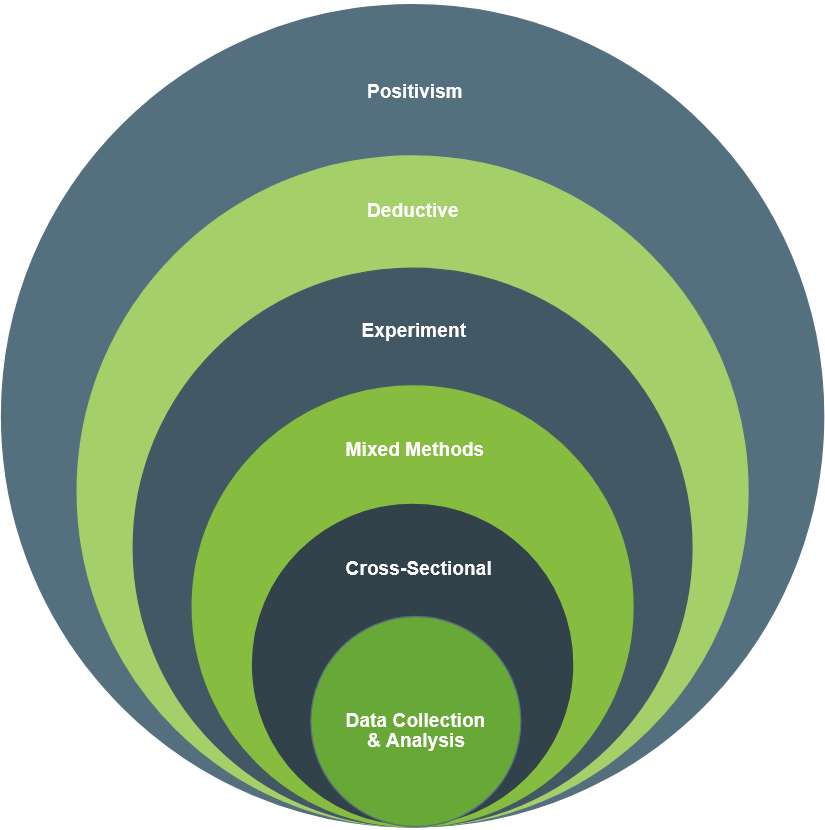
\includegraphics[width=0.45\textwidth]{../Images/Research_Onion.PNG}
    \caption{Research Onion}
    \label{fig:research_onion}
\end{figure}

\subsection{Background to the Research Theme}
Game AI has evolved significantly over the years, especially in RTS games. Early RTS titles, such as StarCraft, relied on Finite State Machines (FSMs) for their AI decision-making. These FSM-based approached
are deterministic and predictable, which can lead to repetitive and boring gameplay, and allow players to exploit the gameplay patters of the AI. \cite{vinyals_grandmaster_2019}

More recently, RL has emerged as an alternative AI approach, taking advantage of advancements in ML and computer hardware. In games such as AlphaStar \cite{vinyals_grandmaster_2019}, RL agents were able to 
demonstrate adaptive and human-like behaviour, providing a more challenging and engaging experience for players. Another paper that highlights this is the work done by Grech \cite{grech_creating_2023}, 
where he created multiple difficulties of AI opponents using RL, and found that players reported higher levels of enjoyment and immersion. A similar study is the one done by \cite{bin_ramlan_implementation_2021},
where they trained an RL agent to act as an opponent in a fighting game, with the agent being able to adapt to the player's skill level, and provide a more engaging experience, similar to the work done by \cite{vinyals_grandmaster_2019}

Despite all of this, the implementation of RL in commercial games remains limited due to the high computational cost, long training and development times, and added complexity. 
This further proves the need for research in this area, and in evaluating if the benefits of RL agents in RTS games are worth the cost compared to traditional FSMs.

\subsection{Hypothesis}

Players report a higher level of enjoyment and improved experience when playing against RL agents comparted to FSMs in RTS games.

\subsection{Independent \& Dependent Variables}

Independent variables are variables that are manipulated by the researcher, and are mainly used to influence the dependant variables. Dependant variables are what happen as a result of the independant variables,
and are what the researcher is interested in measuring.

The independent variable in this study is the type of AI opponent. The dependant variables, those are player experience, player immersion, and perceived difficulty.
Player experience will be measured through surveys and engagement metrics, player immersion will be measured through surveys and validated game design principles, and perceived difficulty will be measured through 
surveys, player feedback, and engagement metrics.

\subsection{Research Aim}

The aim of this study is to evaluate the impact of Reinforcement Learning (RL) and Finite State Machines (FSMs) AI opponents on player experience in Real-Time Strategy (RTS) games, and determine if the extra resources
is justified by the improvement in player experience for RL agents.

To be more specific, the study will focus on the following research objectives:

\begin{itemize}
    \item Compare player-reported enjoyment and engagement levels when playing against RL and FSM AI opponents in RTS games.
    \item Assess the impact of RL and FSM AI opponents on player immersion in RTS games.
    \item Determine if the computational and development costs and complexity of RL justify its implementation over FSMs in RTS games.
\end{itemize}

\subsection{Purpose Statement}

This study is important because AI opponents shaoe the core gameplay experience of RTS games. While FSMs remain widely used due to their simplicity, RL-based AI has the potential to revolutionise
RTS games by providing adaptive and unpredictable opponents. However, the significant resource demand from developers raise questions if the benefits of RL are worth the investment.

By investigating the difference in player experience between RL and FSM AI, this study will provide valuable insights to game developers, AI designers, and the broader gaming community, helping them
in making more informed decisions regarding AI decision-making strategies in RTS game development.

\section{Literature Review}

% The difference between academic and non academic literature is that academic literature is peer-reviewed, and is as such, more reliable and trustworthy
% than non-academic literature, which can easily be biased or contain false information. Academic literature can also be more in-depth and detailed, due to
% the high research standards and requirements of academic institutions, especially IEEE.

% TODO: Filter through the papers in zotero and remove the excessive/unnecessary ones while developing the literature map and review.

Literature review goes here

% Mention Csikszentmihalyi's flow theory and how it relates to player experience and immersion in games.

The goal of a game developer is to create a game that is fun and engaging, and they do this by creating a game that is challenging, but not too challenging.
As Csikszentmihalyi's flow theory states, the goal of a game is to create a state of flow, where the player is fully immersed in the game, and is not
bored, but also not overwhelmed. There are many ways to achieve this, and one of them is through the use of AI opponents. Traditionally, FSMs are
used as AI opponents, as they are simple to implement and easy to understand, and when done correctly, provide a good challenge to the player.
However, given enough time, players can learn the patterns of the FSMs, and exploit them, making the game feel boring. It is possible to combat this
through weakening the player, or making the AI more difficult, as is done in Souls-like games, however this can prove too challenging and overwhelm the player,
once again breaking the flow. 

RL agents, on the other hand, are able to learn how to play the game, and as such, adapt to the player and given scenario. This creates a more engaging
and immersive experience, as the player feels like they are playing against a real opponent, and not just a computer. This is especially true in RTS games,
due to the complexity of the game, and the many strategies that can be taken, which can be seen in the work done by \cite{vinyals_grandmaster_2019}.
There is an issue with this, however, as not only are RL Agents computationally expensive, but they can be trained too far, and become too difficult for the player,
once again breaking the flow state. In the work done by \cite{grech_creating_2023}, they balance this by taking snapshots of the RL agent at different
stages in training. This allows them to create different difficulties of AI opponents, which can be used to better match a player's skill level. 

% Another way of doing this, is by building dynamic difficulty adjustment (DDA) systems into the opponent, which work by adjusting the rewards and punishments
% of the agent to make them easier or harder to play against (Add citation from zotero.).

% Go about comparing these 3 different approaches, and how they always compare the performance of the RL agent, and not the player experience.

\section{Research Methodology}

% Research Questions:

% 1. How do RL and FSM AI opponents compare in terms of player experience in RTS games?
% 2. What are the key factors that influence player experience when playing against RL and FSM AI opponents in RTS games?
% 3. How do RL and FSM AI opponents impact player immersion in RTS games?

% Research objective:

% The objective for the research is to evaluate the impact of RL and FSM opponents in RTS games, and to determin their impact on player experience and immersion,
% and what are the key factors that cause this impact/infuence. This is to be done by creating a simple RTS game, and implementing both RL and FSM agents,
% and then conducting a play test experiment with players, where both groups will then be surveyed to gather data on their experience. Along with this,
% data gathered during the playtest through unity analytics will be used to measure player engagement and immersion.

Research Methodology goes here

\section{Findings}

Findings go here

\section{Conclusion}

Conclusion goes here:

\bibliographystyle{ieeetr}
\bibliography{references}
\end{document}
